% CODHES 2026 Conference Paper
% From Human-Centric to Machine-Optimized: A Technolinguistic Analysis of Documentation Readability in llms.txt Standards
% Compile with: pdflatex -> bibtex -> pdflatex -> pdflatex
%
\documentclass[10pt,conference,a4paper]{IEEEtran}

% ============================================================
% PACKAGES
% ============================================================
\usepackage[T1]{fontenc}
\usepackage[utf8]{inputenc}
\usepackage{times}           % Times New Roman equivalent
\usepackage{microtype}         % Better typography
\usepackage{graphicx}          % Figures
\usepackage{caption}           % Custom captions
\usepackage{booktabs}          % Professional tables
\usepackage{array}             % Extended column types
\usepackage{multirow}          % Multi-row cells
\usepackage{amsmath,amssymb}  % Math
\usepackage{url}               % URL formatting
\usepackage{hyperref}          % Hyperlinks (keep last)

% ============================================================
% PAGE GEOMETRY (matches DOCX: A4, margins ~45pt L/R, 27pt top, 72pt bottom)
% ============================================================
\usepackage[
    a4paper,
    left=45pt,
    right=45pt,
    top=27pt,
    bottom=72pt,
    headheight=36pt,
    footskip=36pt
]{geometry}

% ============================================================
% CUSTOM FORMATTING TO MATCH DOCX TEMPLATE
% ============================================================

% --- Abstract Formatting ---
% DOCX: 9pt bold, justified, first-line indent 13.6pt, spacing after 10pt
\renewcommand{\abstractname}{Abstract}
\renewenvironment{abstract}{%
    \normalfont\fontsize{9pt}{10.8pt}\selectfont\bfseries
    \noindent\ignorespaces
}{%
    \par\addvspace{10pt}%
}

% --- Keywords Formatting ---
% DOCX: italic, indented 13.7pt, spacing after 6pt
\newenvironment{keywords}{%
    \normalfont\itshape\fontsize{10pt}{12pt}\selectfont
    \noindent\hspace{13.7pt}Keywords---\ignorespaces
}{%
    \par\addvspace{6pt}%
}

\makeatletter
% --- Heading Styles (match DOCX specs) ---
% H1: spacing before 8pt, after 4pt
% H2: italic, before 6pt, after 3pt
% H3: italic, exact 12pt line, first indent 14.4pt
% H4: italic, before 2pt, after 2pt, first indent 25.2pt
% H5: before 8pt, after 4pt

\def\section{\@startsection{section}{1}{\z@}{8pt}{4pt}{\normalfont\normalsize\centering\scshape}}
\def\subsection{\@startsection{subsection}{2}{\z@}{6pt}{3pt}{\normalfont\normalsize\itshape}}
\def\subsubsection{\@startsection{subsubsection}{3}{\parindent}{4pt}{2pt}{\normalfont\normalsize\itshape\fontsize{10pt}{12pt}\selectfont}}
\def\paragraph{\@startsection{paragraph}{4}{25.2pt}{2pt}{2pt}{\normalfont\normalsize\itshape}}
\newcounter{subparagraph}[paragraph]
\renewcommand{\thesubparagraph}{\theparagraph.\arabic{subparagraph}}
\renewcommand{\subparagraphmark}[1]{}
\def\subparagraph{\@startsection{subparagraph}{5}{\parindent}{8pt}{4pt}{\normalfont\normalsize\centering\scshape}}
\makeatother

% --- Body Text ---
% DOCX: 10pt, justified, first-line indent 14.4pt, line spacing 11.4pt (auto)
\setlength{\parindent}{14.4pt}

% --- References ---
% DOCX: 8pt, exact 9pt line spacing, justified
\let\oldthebibliography\thebibliography
\let\endoldthebibliography\endthebibliography
\renewenvironment{thebibliography}[1]{%
    \normalfont\fontsize{8pt}{9pt}\selectfont\linespread{1.0}\selectfont
    \oldthebibliography{#1}%
}{%
    \endoldthebibliography
}

% --- Figure and Table Captions ---
% DOCX: 8pt (16 half-points), specific spacing
% Table caption (tablehead style): 8pt small caps, centered, before 12pt after 6pt
% Figure caption (figurecaption style): 8pt italic, justified, before 4pt after 10pt
\captionsetup{font=footnotesize, labelfont={footnotesize,sc}, textfont=footnotesize, justification=centering, skip=6pt}
\captionsetup[table]{position=above, skip=6pt}
\captionsetup[figure]{position=below, skip=4pt}

% --- Table Styles (match DOCX) ---
% DOCX table styles: 8pt for various elements
% Template uses thin grid borders (0.25pt) all around
\setlength{\arrayrulewidth}{0.25pt}

\newcolumntype{C}[1]{>{\centering\arraybackslash}p{#1}}
\newcolumntype{J}[1]{>{\arraybackslash}p{#1}}
\newcolumntype{R}[1]{>{\raggedleft\arraybackslash}p{#1}}

% Table head (centered, 8pt, small caps)
\newcommand{\tablehead}[1]{\multicolumn{1}{c}{\fontsize{8pt}{9.6pt}\selectfont\scshape #1}}
% Table column head (centered, 8pt bold, full cell bordered vertically and horizontally)
\newcommand{\tablecolhead}[1]{%
  \multicolumn{1}{|c|}{\fontsize{8pt}{9.6pt}\selectfont\bfseries #1}%
}
% Table column subhead (centered, 7.5pt italic)
\newcommand{\tablecolsubhead}[1]{\multicolumn{1}{c}{\fontsize{7.5pt}{9pt}\selectfont\itshape #1}}
% Table copy (8pt, justified)
\newcommand{\tablecopy}[1]{\fontsize{8pt}{9.6pt}\selectfont #1}
% Table footnote (6pt, right-aligned)
\newcommand{\tablefootnote}[1]{\vspace{3pt}\par\hfill\fontsize{6pt}{7.2pt}\selectfont #1\par\vspace{1.5pt}}

% ============================================================
% TITLE AND AUTHOR SETUP
% ============================================================

\title{%
    \normalfont\fontsize{24pt}{28.8pt}\selectfont\bfseries
    From Human-Centric to Machine-Optimized: A Technolinguistic Analysis of Documentation Readability in llms.txt Standards%
}

\author{%
    \makebox[\textwidth][c]{%
        \begin{minipage}[t]{0.31\textwidth}
            \centering
            \normalsize Yehezkiel Gunawan\\[3pt]
            \fontsize{8.5pt}{10pt}\selectfont
            Information Systems Department\\
            BINUS Online Learning\\
            Bina Nusantara University\\
            Jakarta, Indonesia\\
            yehezkiel.gunawan@binus.ac.id
        \end{minipage}\hfill
        \begin{minipage}[t]{0.31\textwidth}
            \centering
            \normalsize Tanty Oktavia\\[3pt]
            \fontsize{8.5pt}{10pt}\selectfont
            Information Systems Management Department\\
            BINUS Graduate Program\\
            Bina Nusantara University\\
            Jakarta, Indonesia\\
            toktavia@binus.edu
        \end{minipage}\hfill
        \begin{minipage}[t]{0.31\textwidth}
            \centering
            \normalsize Hadi Syahrial\\[3pt]
            \fontsize{8.5pt}{10pt}\selectfont
            Information Systems Management Department\\
            BINUS Graduate Program\\
            Bina Nusantara University\\
            Jakarta, Indonesia\\
            hadi.syahrial@binus.ac.id
        \end{minipage}%
    }%
}

% Word count: approximately 4,850 body-text words (texcount, excluding verbatim excerpts and references)

% ============================================================
% DOCUMENT BEGINS
% ============================================================
\begin{document}

\maketitle

% Abstract
\begin{abstract}
This study compares human-readable HTML documentation and machine-oriented \texttt{llms.txt} files across ten software engineering platforms. Flesch Reading Ease (FRE), Flesch-Kincaid Grade Level, lexical density, and token-to-word ratio are combined with an LLM-as-a-Judge evaluation and a preliminary LLM Readability Index (LRI). Machine documentation had a 91.58-point lower mean FRE but a 14.69-point higher mean LRI ($p=0.005$, $d=-1.172$). Clarity, completeness, conciseness, and LLM-friendliness favored machine documentation with large effects; Technical Accuracy did not differ significantly. No statistically significant correlation was detected between traditional readability metrics and LLM ratings. These findings identify a readability-tokenization paradox in measurement outcomes: formats rated favorably by the selected evaluator can score poorly on human-oriented readability formulas. LRI is an operational composite, not a validated readability instrument, and the study does not establish improved downstream LLM performance.
\end{abstract}

% Keywords
\begin{keywords}
technolinguistics, documentation readability, LLM-as-a-Judge, llms.txt, Flesch Reading Ease, LLM Readability Index, technical documentation, tokenization
\end{keywords}

\IEEEpeerreviewmaketitle

\linespread{0.95}\selectfont

% ============================================================
% INTRODUCTION
% ============================================================
\section{Introduction}

LLM-based assistants increasingly mediate access to software engineering documentation, creating a second audience alongside human developers. Human-oriented documentation is typically organized and evaluated for comprehension, whereas machine-oriented formats favor compact, structured access within finite context windows. This raises a measurement question: do formats designed for machine consumption trade traditional readability for qualities that an LLM evaluator rates more favorably?

Readability has long guided technical communication. FRE and FKGL operationalize difficulty through sentence length and syllable counts and remain embedded in widely used writing tools. Those formulas, however, were calibrated for human readers and continuous prose. They do not account for navigation, retrieval structure, code, Markdown syntax, or the needs of an LLM consuming documentation as context. Applying them unchanged to machine-oriented files may therefore conflate linguistic difficulty with structural difference.

Jeremy Howard introduced the \texttt{llms.txt} standard in September 2024 as a compact, Markdown-based source for inference-time use. Its emergence parallels earlier changes from print to HTML, but established readability formulas were designed for continuous human prose rather than link directories, API listings, or token-oriented structures. Byte Pair Encoding further complicates evaluation because vocabulary and markup affect token cost independently of sentence-level readability. The ``Lost in the Middle'' effect also motivates concise, front-loaded access to documentation \cite{Liu2023}.

Developer-facing AI assistants now retrieve documentation to answer questions, explain APIs, and support coding tasks. This use makes documentation quality consequential, but it does not follow that a file labeled for LLM use improves those tasks. A measurement design must separate traditional readability, tokenization behavior, evaluator preference, and downstream performance. The present study addresses the first three and treats the fourth as an external-validation requirement.

This study addresses the gap through a quantitative, platform-matched paired comparison of human-readable HTML and machine-oriented documentation from ten software engineering platforms. The sample spans frameworks, developer platforms, infrastructure, payments, AI tools, and backend services. Traditional readability and tokenization measures are compared with five LLM-as-a-Judge dimensions and a preliminary composite LRI. Platform matching supports within-platform comparison but does not imply that paired corpora are content-identical.

The contribution is threefold: empirical comparison of human- and machine-oriented documentation, measurement of the divergence between traditional metrics and LLM ratings, and a reproducible framework for examining this divergence. The resulting readability-tokenization paradox concerns measurement outcomes rather than demonstrated gains in retrieval, generation, or user performance.

% ============================================================
% RESEARCH QUESTIONS
% ============================================================
\subsection{Research Questions}

This study addresses three primary research questions:

\textbf{RQ1:} Do machine-oriented documentation files (\texttt{llms.txt}) have markedly different traditional readability scores than their human-readable HTML counterparts?

\textbf{RQ2:} Do the LLM-as-a-Judge evaluation scores favor machine-oriented documentation over human-readable HTML documentation?

\textbf{RQ3:} Are existing readability measures (Flesch Reading Ease, Flesch-Kincaid Grade Level) sufficient for assessing documentation meant for both human and machine consumption, or do they fail to reflect LLM-perceived quality dimensions?

% ============================================================
% SIGNIFICANCE
% ============================================================
\subsection{Significance of the Study}

This study contributes to technolinguistics by quantifying how human-oriented readability formulas and LLM-based quality ratings diverge. It offers documentation teams a basis for complementary evaluation while positioning LRI as a preliminary composite requiring external validation.

% ============================================================
% LITERATURE REVIEW
% ============================================================
\section{Literature Review}

\subsection{The llms.txt Standard and Machine-Oriented Documentation}

Howard proposed \texttt{llms.txt} to provide LLMs with concise, structured website information at inference time \cite{Howard2024}. The Markdown format uses a title, summary, curated links, and an optional section whose content can be omitted under tighter context constraints. It therefore separates machine access from HTML navigation, advertising, and client-side presentation. Vercel, Cloudflare, Postman, Cursor, Anthropic, and Hugging Face are among its adopters \cite{AnswerDotAI2024}; related tools generate the format for major documentation systems, while variants such as \texttt{llms-full.txt} aggregate fuller content \cite{llmstxtSite,llmstxtDirectory}. This ecosystem makes explicit the tension examined here: a document can be concise and structured for machine access without satisfying conventions developed for human prose.

The proposal responds to a practical retrieval problem: converting complex websites with navigation and JavaScript into plain text is noisy, while placing an entire site in context is often infeasible. A curated root file can expose summaries and links, and a fuller variant can aggregate source material for systems with larger budgets. Implementations nevertheless vary substantially. Some sites provide short indexes, others publish prose-rich topic collections, and others expose very large aggregates. Thus, \texttt{llms.txt} denotes an access convention rather than a uniform textual genre.

\subsection{Traditional Readability Metrics}

The Flesch Reading Ease (FRE) formula, developed by Rudolf Flesch in 1948 \cite{Flesch1948}, and the Flesch-Kincaid Grade Level (FKGL), developed by J. Peter Kincaid et al. in 1975 \cite{Kincaid1975}, are the foundation of modern readability measurement. The FRE formula uses sentence length and syllable count per word to compute readability; FKGL converts these metrics into U.S. grade level equivalents.

These formulas have gained academic credibility. Flesch's original research appeared in the Journal of Applied Psychology, and FKGL became a U.S. military standard in 1978. The U.S. Department of Defense, Microsoft Word, Grammarly, and IBM Lotus Symphony have all adopted these measures. Yet Redish (2000) \cite{Redish2000} and McClure (1987) \cite{McClure1987} point out serious limitations when applying these formulas to technical documentation: they were built for schoolbooks, not technical content; they ignore reader differences and the effects of content, layout, and retrieval aids; and they assume English text, limiting their applicability to non-English contexts.

Industry standards for technical documentation suggest grade levels of 8-10 for general developer audiences and FRE scores of 60-70 for general documentation \cite{Kincaid1988}. Technical content often scores lower because readability formulas penalize polysyllabic terminology. This limitation matters for machine-oriented documentation, which may use dense, concise language that traditional metrics rate as less readable.

Alternative formulas such as ARI, Coleman-Liau, SMOG, and Gunning Fog vary their treatment of vocabulary and sentence complexity but remain surface-based and human-centered. Coh-Metrix adds cohesion and semantic overlap at greater computational cost. Neural models can capture context, yet models trained on human judgments retain a human-oriented target. Applying any of these measures to concise instructions, link directories, and API listings is therefore uncertain. This study treats LRI as complementary to, rather than equivalent to, human readability measures.

This construct distinction is important in technical domains. Long identifiers and polysyllabic product terms can depress formula scores even when they are familiar to the intended audience. Conversely, a short link label can appear linguistically simple while providing insufficient context. Layout, prior knowledge, examples, and retrieval aids also shape human comprehension but are absent from FRE and FKGL. The metrics remain useful as standardized surface indicators, provided their outputs are not interpreted as direct comprehension measurements for non-prose artifacts.

\subsection{Tokenization and Computational Efficiency}

Byte Pair Encoding (BPE), introduced to NLP by Sennrich, Haddow, and Birch in 2016 \cite{Sennrich2016}, is the standard tokenization method for modern LLMs. BPE is lossless, reversible, and compresses text, typically producing tokens of about 4 bytes each \cite{OpenAI2023}. Variable-length encoding is its key feature: common words need only one token, while rare or complex words need several. Recent work has examined how tokenization choices affect model behavior \cite{Ankner2024}, and the selection of subword merge operations has a notable effect on downstream performance \cite{Ding2019}.

Token count affects API cost, latency, and context-window use. The ``Lost in the Middle'' phenomenon, in which models use information less reliably when it appears within long contexts, motivates concise and front-loaded formats such as \texttt{llms.txt} \cite{Liu2023}.

Token efficiency is not equivalent to brevity in words. Rare technical terms, URL fragments, punctuation, and Markdown can split into multiple tokens, so a compact directory may have a high TWR even when it contains little prose. TWR is included to expose this computational property without treating it as a direct measure of model comprehension or task success.

LLMLingua (Jiang et al., 2023), published at EMNLP 2023, demonstrates that well-structured compression can preserve semantic integrity while reducing token count \cite{Jiang2023}, achieving up to 20x prompt compression with minimal performance loss. This work, however, focuses on compression techniques rather than documentation standards. It leaves a gap in the understanding of how documentation format choices affect machine efficiency and human readability.

\subsection{LLM-as-a-Judge Evaluation Methodology}

LLM-as-a-Judge methods assess semantic qualities that formula-based metrics omit, including clarity, completeness, conciseness, and technical accuracy. Strong judges can exceed 80\% agreement with human preferences in some settings \cite{Zheng2023}, and related work has applied LLM evaluation to code readability \cite{Horikawa2026,Simoes2025} and generated documentation \cite{Diggs2024}. These results support scalable evaluation but do not remove model-specific bias or establish downstream utility.

Judge outputs depend on the selected model, rubric, prompt, scale, and aggregation procedure. Position bias, score compression, and self-preference have been documented in adjacent evaluation settings. For this reason, the five dimensions in this study are reported individually as well as through LRI, and Technical Accuracy is not assumed to behave like presentation-oriented dimensions.

\subsection{Research Gap}

Despite the extensive literature on readability metrics, tokenization efficiency, and LLM evaluation, a key gap remains: no peer-reviewed study has systematically compared traditional readability metrics with LLM evaluation scores for machine-oriented documentation. This study addresses that gap across ten technical documentation platforms.

% ============================================================
% METHOD
% ============================================================
\section{Method}

\subsection{Research Design}

This study uses quantitative content analysis and a platform-matched paired design. Human-readable HTML documentation and machine-oriented files from the same platforms are compared using traditional computational-linguistics metrics and an LLM-as-a-Judge evaluation. Platform matching reduces domain variation but does not make the paired corpora content-identical.

The platform is the unit of pairing. Scores were aggregated within each platform and documentation type before paired inference, avoiding treatment of chunks as independent platform observations. The design supports comparison of formats as they existed in practice; it does not isolate format from differences in coverage, implementation maturity, or source composition.

\subsection{Corpus Selection}

The corpus includes ten software engineering documentation platforms selected for their adoption of \texttt{llms.txt}-style documentation and representation of diverse technical domains. Selection required (1) human-readable HTML and machine-oriented documentation, (2) a technical rather than marketing focus, (3) English content, and (4) public accessibility.

Purposive selection provided variation across frontend and backend frameworks, developer and deployment platforms, infrastructure, payments, AI orchestration, and backend services. This diversity reduces dependence on a single software domain, but it does not support population-level estimates for all technical documentation. Table~\ref{tab:platforms} describes the sample.

\begin{table}[t]
    \caption{Platform Characteristics}
    \label{tab:platforms}
    \begin{tabular}{|J{2.5cm}|J{2.9cm}|J{2cm}|}
        \hline
        \tablecolhead{Platform} & \tablecolhead{Category} & \tablecolhead{Domain} \\
        \hline
        \tablecopy{React} & \tablecopy{UI Framework} & \tablecopy{Frontend} \\
        \hline
        \tablecopy{GitHub} & \tablecopy{Developer Platform} & \tablecopy{DevOps} \\
        \hline
        \tablecopy{Supabase} & \tablecopy{Backend-as-a-Service} & \tablecopy{Backend} \\
        \hline
        \tablecopy{Vercel} & \tablecopy{Deployment Platform} & \tablecopy{DevOps} \\
        \hline
        \tablecopy{Stripe} & \tablecopy{Payment Platform} & \tablecopy{Fintech} \\
        \hline
        \tablecopy{LangChain} & \tablecopy{AI Orchestration} & \tablecopy{AI/ML} \\
        \hline
        \tablecopy{Cloudflare} & \tablecopy{Infrastructure} & \tablecopy{DevOps} \\
        \hline
        \tablecopy{Cursor} & \tablecopy{AI Editor} & \tablecopy{Developer Tools} \\
        \hline
        \tablecopy{Hono} & \tablecopy{Web Framework} & \tablecopy{Backend} \\
        \hline
        \tablecopy{FastAPI} & \tablecopy{Python Framework} & \tablecopy{Backend} \\
        \hline
    \end{tabular}
\end{table}

\subsection{Data Collection}

Data were collected with a custom Python CLI that separates acquisition, cleaning, measurement, evaluation, and export. For the human corpus, Crawl4AI and Playwright performed breadth-first crawling to a maximum depth of three and 50 pages per platform, including JavaScript-rendered sites. Mozilla Readability extracted prose into Markdown; navigation, code blocks, images, advertisements, and scripts were removed while headings, paragraphs, and link anchors were retained \cite{MozillaReadability}. Cleaned outputs below 500 characters were flagged for alternative extraction or manual review.

The crawler restricted traversal to documentation-relevant pages and converted rendered HTML to Markdown before prose extraction. Removing code prevents source listings from dominating sentence and lexical calculations, but this choice also means that the human corpus represents explanatory prose rather than every element visible on the original page. Headings and anchors were retained because they contribute to how readers identify and retrieve topics.

The machine corpus was assembled by checking each root domain for \texttt{/llms.txt} and the legacy \texttt{/llm.txt} endpoint, then following linked text files in their listed order. Expanded variants such as \texttt{llms-full.txt} and \texttt{llms-ctx.txt} were included when available. Context7 supplied fallback content when no direct file existed or when it returned a more complete source. Human files averaged approximately 150,000 characters per platform, whereas machine files ranged from 3,000 to 8.8 million characters, reflecting variation from concise summaries to full-documentation aggregates. Appendix A shows representative excerpts.

Relative links were resolved against each platform domain, and linked text files were concatenated in source order. When Context7 was considered, content length determined whether its version replaced the direct source. This rule favored coverage but did not guarantee topical equivalence with the crawled human pages. Source files were retained so that corpus construction and the structural heterogeneity visible in Appendix A could be inspected.

Long documents were divided into approximately 4,000-token chunks. The model \texttt{nvidia/nemotron-nano-12b-v2-vl} evaluated each chunk through OpenRouter \cite{OpenRouter2024} using a structured prompt and JSON response schema; dimension scores were averaged equally across chunks. Cached responses supported resumable processing. Figure~\ref{fig:pipeline} summarizes the collection and analysis flow.

The prompt supplied definitions and a 1--5 rubric for every dimension and required parseable scores. Temperature was set to 0.0 to reduce stochastic variation. Each chunk contributed equal weight to the platform score, including a shorter final chunk; this choice simplified aggregation but is treated as a limitation. The model was selected to keep the procedure accessible and reproducible rather than to claim evaluator consensus.

\begin{figure*}[!t]
    \centering
    \fbox{\parbox{0.9\textwidth}{
    \centering
    \small
    \textbf{Data Collection and Analysis Pipeline}\\[6pt]
    \begin{tabular}{ccc}
        \textbf{Input} & $\rightarrow$ & \textbf{Detection} \\
        (urls.txt) & & (llms.txt check) \\[6pt]
        & & $\downarrow$ \\[6pt]
        \textbf{Export} & $\leftarrow$ & \textbf{Metrics} \\
        (CSV/MD/Raw) & & (FRE/FKGL/LD) \\[6pt]
        & & $\uparrow$ \\[6pt]
        \textbf{LLM Eval} & $\rightarrow$ & \textbf{Clean} \\
        (5 Dimensions) & & (Prose Extraction) \\[6pt]
        & & $\uparrow$ \\[6pt]
        \textbf{LRI Calc} & $\leftarrow$ & \textbf{Crawl} \\
        (0-100 Scale) & & (Human Docs) \\
    \end{tabular}
    }}
    \caption{Data Collection and Analysis Pipeline showing the flow from input URLs through detection, crawling, cleaning, metrics calculation, and LLM evaluation to final export.}
    \label{fig:pipeline}
\end{figure*}

\subsection{Metrics and Instruments}

\subsubsection{Traditional Readability Metrics}

The study uses three traditional readability metrics implemented with the Python textstat library:

\textbf{Flesch Reading Ease (FRE):} Calculated as $206.835 - 1.015(\text{total words} / \text{total sentences}) - 84.6(\text{total syllables} / \text{total words})$. Scores range from 0 to 100, with higher scores indicating easier readability.

\textbf{Flesch-Kincaid Grade Level (FKGL):} Calculated as $0.39(\text{total words} / \text{total sentences}) + 11.8(\text{total syllables} / \text{total words}) - 15.59$. Scores represent U.S. grade level equivalents.

\textbf{Lexical Density (LD):} Calculated as the percentage of content words (nouns, verbs, adjectives, adverbs) relative to total words, using the NLTK stopwords corpus for stopword identification.

\textbf{Token-to-Word Ratio (TWR):} Calculated using OpenAI's tiktoken library with the cl100k\_base encoding (GPT-4). This metric measures the ratio of tokens to words, indicating tokenization efficiency.

\subsubsection{LLM-as-a-Judge Evaluation}

The LLM evaluation uses a five-dimension Likert scale assessment via the OpenRouter API \cite{OpenRouter2024}, using the nvidia/nemotron-nano-12b-v2-vl model. The evaluation dimensions are:

\begin{enumerate}
    \item \textbf{Clarity} (1-5): Is the documentation clear and unambiguous?
    \item \textbf{Completeness} (1-5): Does it cover the topic adequately?
    \item \textbf{Conciseness} (1-5): Is it free of unnecessary verbosity?
    \item \textbf{Technical Accuracy} (1-5): Are technical details correct?
    \item \textbf{LLM-Friendliness} (1-5): Is it optimized for machine consumption?
\end{enumerate}

\textbf{LLM Readability Index (LRI):} The LRI is proposed as a preliminary operational composite of LLM-perceived documentation quality. Let $s_{ij}$ denote the score assigned to document $i$ on dimension $j$, where $s_{ij}\in[1,5]$. The equally weighted mean score is:

\begin{equation}
    \bar{s}_i = \frac{1}{5}\sum_{j=1}^{5}s_{ij}
\end{equation}

The mean is then linearly normalized from the 1--5 range to a 0--100 range:

\begin{equation}
    \mathrm{LRI}_i = 100\left(\frac{\bar{s}_i-1}{5-1}\right) = 25(\bar{s}_i-1)
\end{equation}

Equal weights are assigned because no validated empirical basis currently exists for differential weighting of the five dimensions. The transformation yields 0 when all dimension scores are 1, 50 when their mean is 3, and 100 when all scores are 5. It preserves rankings and inferential conclusions while providing a common numerical range for presentation. Sharing a 0--100 range with Flesch Reading Ease does not imply that the two measures represent equivalent constructs; LRI reflects the evaluator's composite assessment, whereas Flesch Reading Ease reflects surface-level linguistic complexity.

\subsection{Analysis Procedure}

\subsubsection{Statistical Tests}

The analysis uses paired samples t-tests to compare human-readable and machine-oriented documentation for the same platforms. Effect sizes are calculated using Cohen's d for paired samples:

\begin{equation}
    d = \frac{\text{mean difference}}{\text{standard deviation of differences}}
\end{equation}

Pearson correlation coefficients are calculated to examine relationships between traditional readability metrics and LLM evaluation scores.

All tests used two-sided $\alpha=0.05$. Means and standard deviations summarize format-level distributions, and medians and trimmed analyses assess sensitivity to extreme FRE and TWR observations. Statistical significance and effect magnitude are interpreted separately, particularly for Technical Accuracy and the correlation analysis.

\subsubsection{Software and Tools}

Python 3.11+, \texttt{textstat}, \texttt{tiktoken} (\texttt{cl100k\_base}), NLTK, SciPy, pandas, NumPy, Matplotlib, and seaborn supported measurement, analysis, and visualization. A standalone analysis script reads exported CSV data and regenerates the statistical tables and reports.

\subsubsection{Validation Steps}

Validity checks covered five areas. First, random samples were compared across raw pages, cleaned Markdown, and metric inputs to assess extraction quality. Second, manual FRE and FKGL calculations for FastAPI, React, and Stripe differed by less than 0.5\% from automated results. Third, robust statistics and trimmed means assessed the influence of React ($\mathrm{FRE}=-430.09$) and LangChain ($-234.73$); removing them changed mean machine FRE from $-58.18$ to $12.45$ without reversing the format-level direction. Fourth, cached outputs preserve the evaluated scores and provenance, although fresh API calls may vary. Finally, re-evaluation of five document pairs one week later produced $r=0.94$, indicating high temporal consistency for the selected judge. Automated tests additionally covered acquisition, cleaning, measurement, evaluation, and export behavior.

Manual inspection focused on whether navigation was removed without discarding the principal explanatory content. Metric checks applied the published formulas to 500-word samples before comparison with automated outputs. The sensitivity analysis is especially important because negative FRE values are mathematically possible but become difficult to interpret when sentence boundaries are sparse. The temporal consistency check measures repeatability for this evaluator and sample; it is not inter-model agreement or external construct validation.

\subsection{AI Declaration}

AI was used for the LLM-as-a-Judge evaluation following established protocols \cite{Zheng2023}, for assistance with analysis code and visualization, and for literature retrieval. The primary author retained control of research design, interpretation, and conclusions.

% IEEEtran delays full-width floats by at least one output cycle; queue these
% here so they appear beside the opening Results discussion on the next page.
\begin{figure*}[!t]
    \centering
    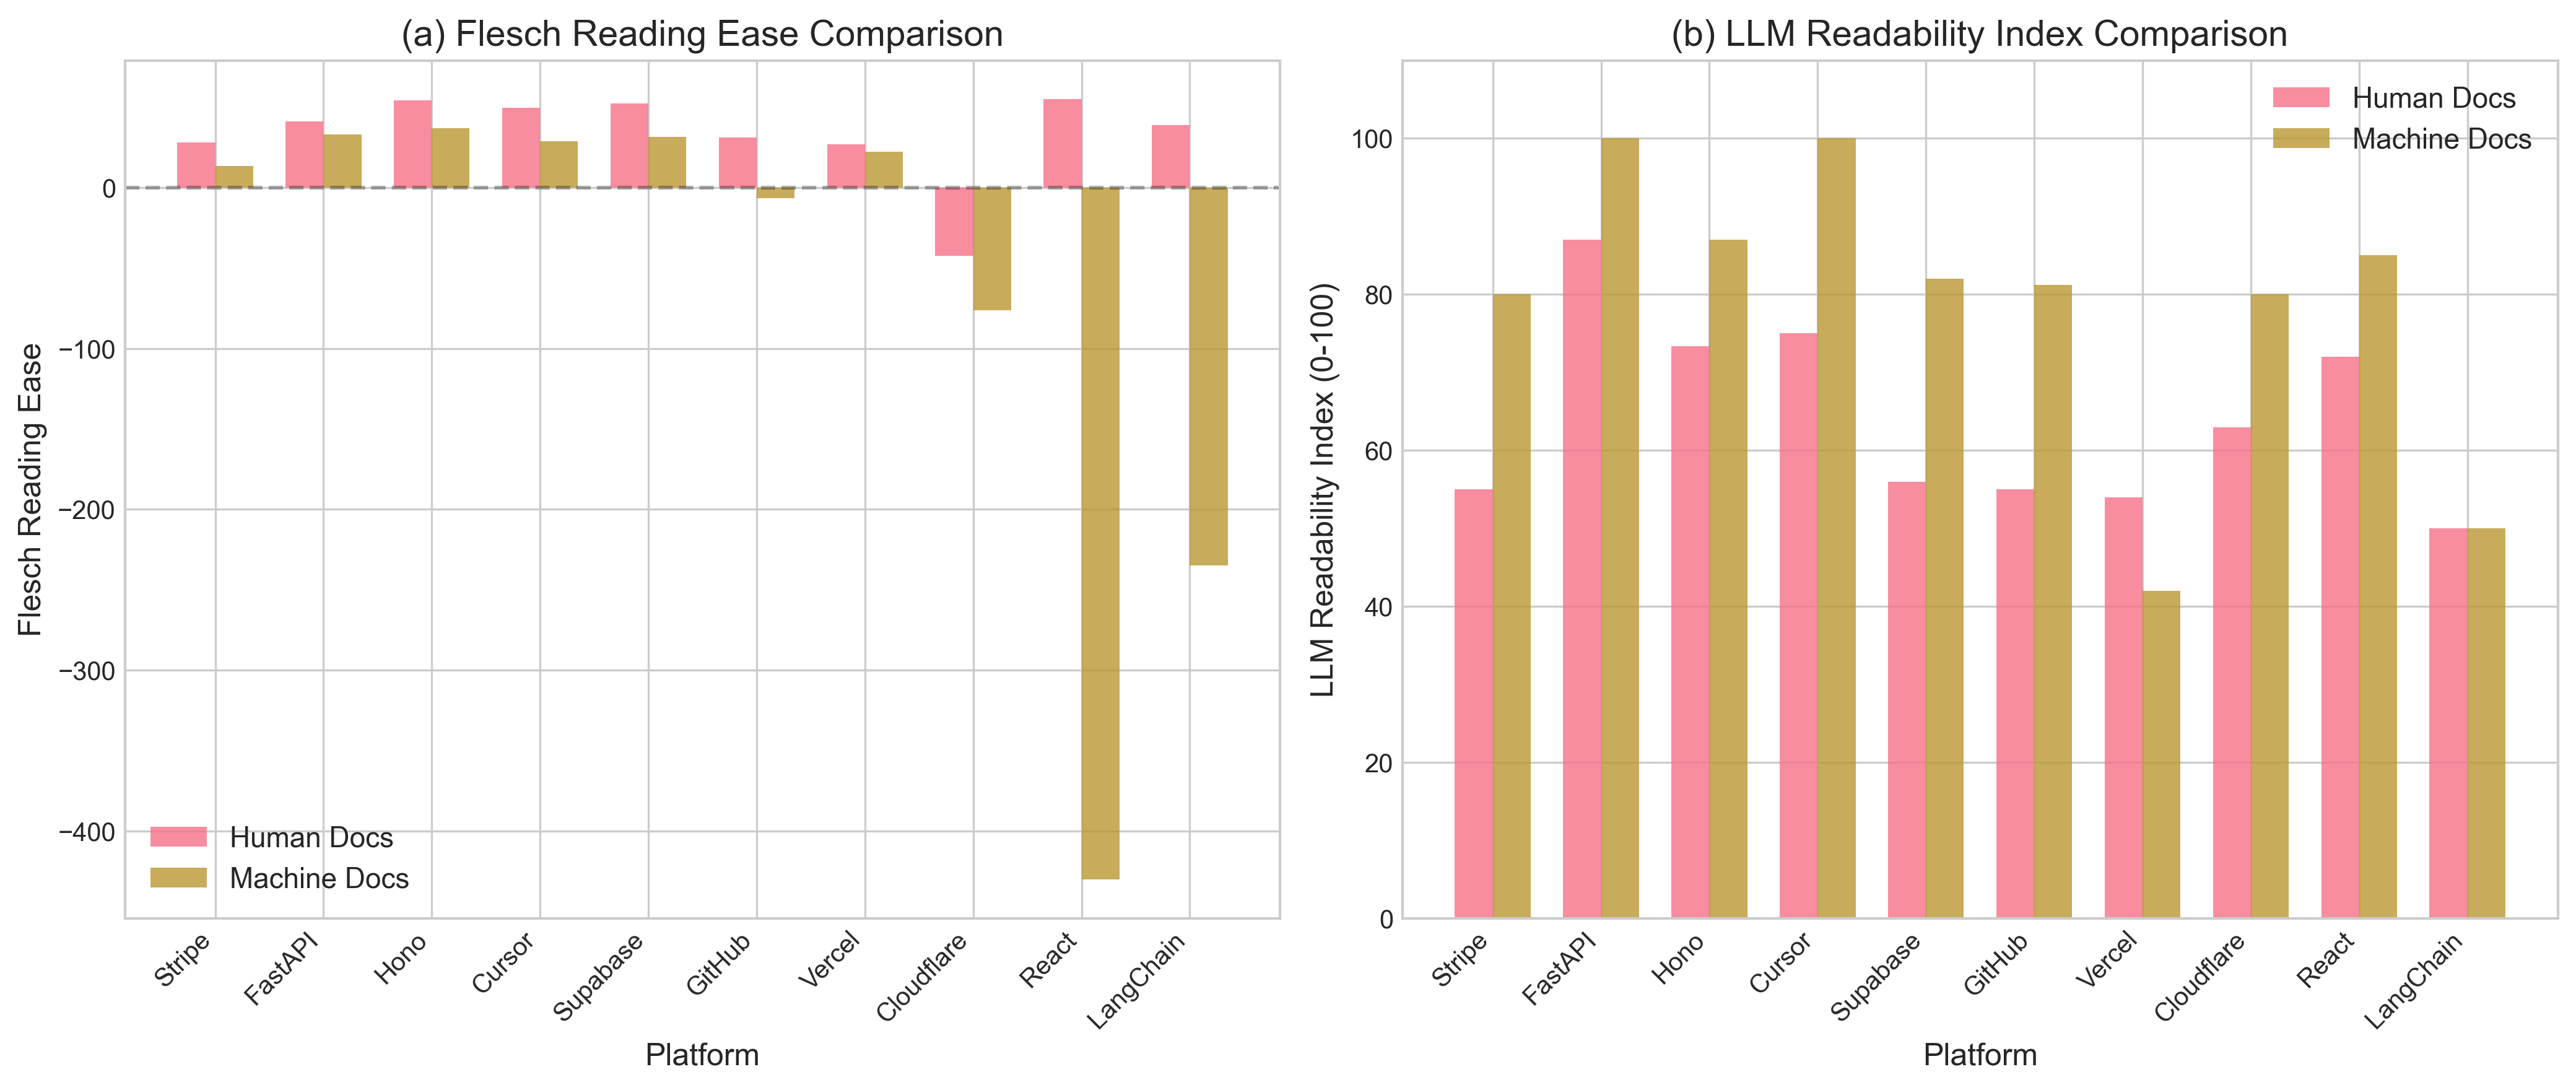
\includegraphics[width=0.9\textwidth]{readability-python-demo/results/figures/figure1_readability_comparison.png}
    \caption{Platform-level comparison of (a) Flesch Reading Ease and (b) LLM Readability Index scores. Human documentation (pink) generally has higher FRE, while machine documentation (gold) generally has higher LRI. React and LangChain illustrate the extreme variance in machine FRE.}
    \label{fig:readability}
\end{figure*}

\begin{table*}[!t]
    \caption{Traditional Readability Metrics Comparison}
    \label{tab:traditional}
    \centering
    \begin{tabular}{|J{3.5cm}|R{2.5cm}|R{2.5cm}|R{1.8cm}|J{1.8cm}|}
        \hline
        \tablecolhead{Metric} & \tablecolhead{Human} & \tablecolhead{Machine} & \tablecolhead{Cohen's d} & \tablecolhead{Effect} \\
        \hline
        \tablecopy{Flesch Reading Ease} & \tablecopy{33.39 (28.66)} & \tablecopy{-58.18 (155.28)} & \tablecopy{0.573} & \tablecopy{Medium} \\
        \hline
        \tablecopy{Flesch-Kincaid Grade} & \tablecopy{13.76 (6.18)} & \tablecopy{23.96 (20.91)} & \tablecopy{-0.459} & \tablecopy{Small} \\
        \hline
        \tablecopy{Lexical Density (\%)} & \tablecopy{76.86 (9.23)} & \tablecopy{77.25 (8.70)} & \tablecopy{-0.028} & \tablecopy{Negligible} \\
        \hline
        \tablecopy{Token-to-Word Ratio} & \tablecopy{1.67 (0.36)} & \tablecopy{2.73 (1.48)} & \tablecopy{-0.661} & \tablecopy{Medium} \\
        \hline
    \end{tabular}
    \tablefootnote{Values are mean (SD). Cohen's d calculated for paired samples. Negative d indicates machine docs score higher than human docs.}
\end{table*}

% ============================================================
% RESULT AND DISCUSSION
% ============================================================
\section{Result and Discussion}

\subsection{Traditional Readability Analysis}

The ten platform pairs span frameworks, services, developer tools, and AI platforms. Figure~\ref{fig:readability} contrasts FRE and LRI: human documentation generally has higher FRE, whereas machine documentation generally has higher LRI. React and LangChain are extreme machine-FRE outliers.

Table~\ref{tab:traditional} shows mixed traditional-metric outcomes. Human documentation has a 91.58-point higher mean FRE, but machine scores vary widely ($SD=155.28$), driven partly by link-heavy React ($-430.09$) and LangChain ($-234.73$) files for which prose-based formulas have weak construct validity. Machine documentation also has a 10.2-level higher mean FKGL. Lexical density is nearly equal across formats, while mean TWR is higher for machine documentation (2.73 versus 1.67), contrary to a simple token-efficiency expectation. React and LangChain exceed 5.0 TWR, showing that implementation structure strongly affects tokenization.

The direction of FRE favors human documentation with a medium paired effect ($d=0.573$), whereas the FKGL effect is smaller ($d=-0.459$). Because the inferential tests for these traditional metrics are not reported, these differences are interpreted descriptively rather than as statistically significant format effects. The near-zero lexical-density effect ($d=-0.028$) indicates that the formats contain similar proportions of content-bearing words even though their sentence structure and markup differ.

The TWR pattern also qualifies the premise that machine-oriented files are inherently token-efficient. A ratio counts token fragments per whitespace-delimited word, not total context length or useful information per token. URLs, punctuation, identifiers, and Markdown links can raise the ratio, while a longer prose document may still contain more tokens overall. TWR therefore identifies one aspect of computational representation rather than an overall efficiency score.

\subsection{LLM-as-a-Judge Evaluation Results}

The selected evaluator rated machine documentation higher on LRI (M=78.72) than human documentation (M=64.03), a mean difference of 14.69 points ($t=-3.706$, $p=0.005$, $d=-1.172$, 95\% CI [4.89, 24.49]). Conciseness ($p=0.006$), LLM-Friendliness ($p=0.007$), Completeness ($p=0.014$), and Clarity ($p=0.015$) also favored machine documentation with large effects. Technical Accuracy showed only a small, non-significant difference ($d=-0.245$, $p=0.455$). Table~\ref{tab:llm} reports the dimension-level results, and Figure~\ref{fig:effect} summarizes the effect sizes without implying downstream performance.

\begin{table*}[!t]
    \caption{LLM-as-a-Judge Evaluation Results}
    \label{tab:llm}
    \centering
    \begin{tabular}{|J{3.5cm}|R{2.5cm}|R{2.5cm}|R{1.8cm}|J{1.8cm}|}
        \hline
        \tablecolhead{Dimension} & \tablecolhead{Human} & \tablecolhead{Machine} & \tablecolhead{Cohen's d} & \tablecolhead{Effect} \\
        \hline
        \tablecopy{Clarity} & \tablecopy{3.50 (0.51)} & \tablecopy{4.08 (0.71)} & \tablecopy{-1.002} & \tablecopy{Large} \\
        \hline
        \tablecopy{Completeness} & \tablecopy{3.38 (0.51)} & \tablecopy{4.01 (0.78)} & \tablecopy{-0.964} & \tablecopy{Large} \\
        \hline
        \tablecopy{Conciseness} & \tablecopy{3.38 (0.58)} & \tablecopy{4.14 (0.81)} & \tablecopy{-1.347} & \tablecopy{Large} \\
        \hline
        \tablecopy{Technical Accuracy} & \tablecopy{4.20 (0.59)} & \tablecopy{4.36 (0.89)} & \tablecopy{-0.245} & \tablecopy{Small} \\
        \hline
        \tablecopy{LLM-Friendliness} & \tablecopy{3.35 (0.58)} & \tablecopy{4.16 (0.82)} & \tablecopy{-1.371} & \tablecopy{Large} \\
        \hline
        \tablecopy{\textbf{LRI (Overall)}} & \tablecopy{\textbf{64.03 (12.13)}} & \tablecopy{\textbf{78.72 (18.88)}} & \tablecopy{\textbf{-1.172}} & \tablecopy{\textbf{Large}} \\
        \hline
    \end{tabular}
    \tablefootnote{Values are mean (SD) on 1-5 Likert scale. LRI = LLM Readability Index (0-100). Negative Cohen's d indicates machine docs score higher.}
\end{table*}

The dimension pattern localizes the aggregate difference. Conciseness ($d=-1.347$) and LLM-Friendliness ($d=-1.371$) show the largest effects, followed by Clarity ($d=-1.002$) and Completeness ($d=-0.964$). These are presentation- and access-oriented criteria that the \texttt{llms.txt} convention explicitly targets. Technical Accuracy remains high in both formats (4.20 human and 4.36 machine), and its non-significant difference provides no evidence that either format is more correct.

\begin{figure*}[!t]
    \centering
    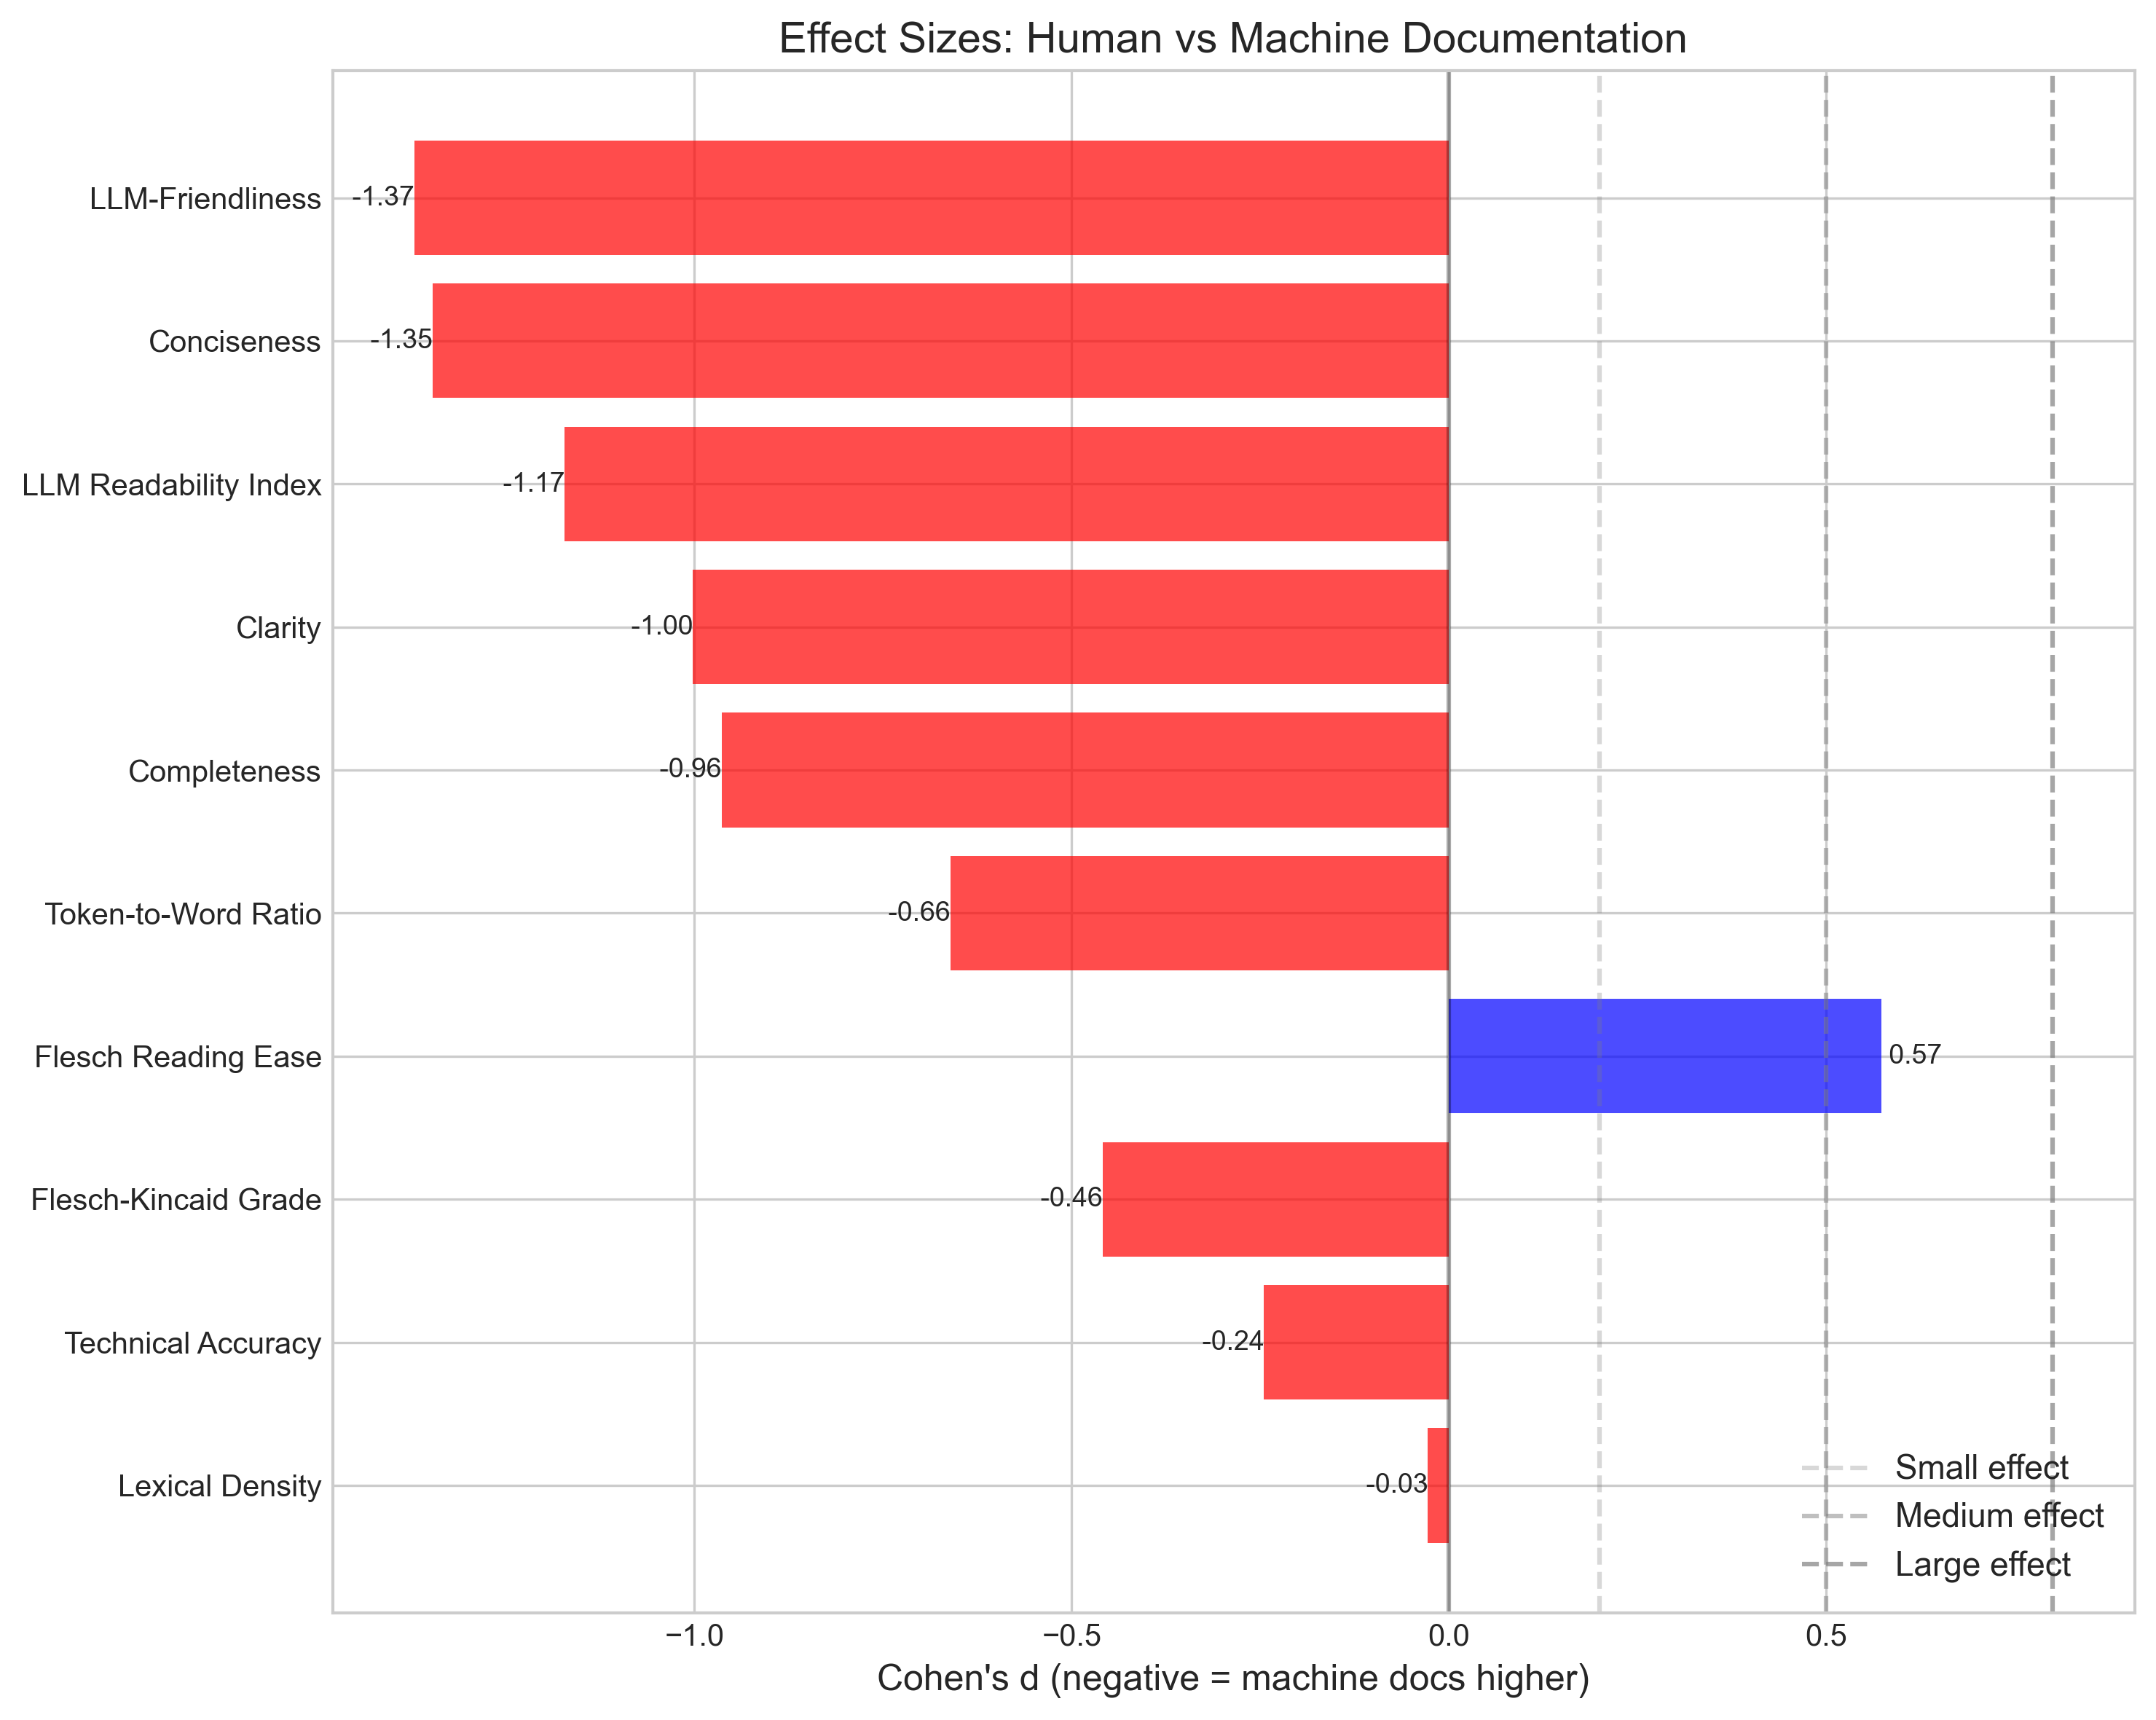
\includegraphics[width=0.72\textwidth]{readability-python-demo/results/figures/figure5_effect_sizes.png}
    \caption{Cohen's d effect sizes for all metrics and evaluation dimensions. Negative values favor machine documentation and positive values favor human documentation. Clarity, Completeness, Conciseness, LLM-Friendliness, and LRI show large machine-favoring effects; Technical Accuracy shows a small effect.}
    \label{fig:effect}
\end{figure*}

Eight of ten platform pairs favor machine documentation. Vercel is the only exception (42.00 machine versus 54.00 human), while LangChain is tied at 50.00. FastAPI and Cursor reach the scale ceiling of 100.00, suggesting potential score compression. Positive deltas range from 13.00 for React and FastAPI to 26.25 for GitHub. This spread, together with Vercel's negative delta, indicates substantial platform-level heterogeneity and shows that format labels alone do not determine evaluator ratings.

\subsection{Correlation Analysis}

No statistically significant correlation was detected between traditional metrics and LLM ratings (all $p>0.05$). FRE and LLM-Friendliness showed $r=0.357$ ($p=0.312$); TWR and LLM-Friendliness showed the largest observed coefficient, $r=0.564$ ($p=0.090$), which fell to $r=0.312$ ($p=0.412$) after removing the React and LangChain TWR outliers. Low-FRE machine files could still receive high Clarity ratings, illustrating divergence between the measures, but the small sample does not establish independence between constructs.

\subsection{The Readability-Tokenization Paradox}

The readability-tokenization paradox describes the observed divergence between human-oriented formulas and LLM-based ratings: machine documentation generally received lower FRE and higher LRI. This is not proof that machines process difficult text more effectively. FRE and FKGL respond to sentence length and syllables, whereas the judge considered broader documentation qualities; TWR separately captures tokenizer fragmentation and markup overhead. Complementary measures are therefore needed for dual-audience documentation.

The term ``paradox'' denotes competing evaluation outcomes, not a logical contradiction. Machine-oriented files can contain dense labels, URLs, and fragments that violate assumptions of prose formulas while presenting a compact hierarchy that the judge rewards for clarity or conciseness. Human files can provide explanation, narrative transitions, and examples that support comprehension while receiving lower conciseness ratings. Neither outcome alone establishes which document better supports a reader or application.

This distinction also explains why higher mean TWR does not negate higher LRI. LRI includes the evaluator's judgments of organization and coverage, whereas TWR reflects lexical segmentation. A file can be fragmented at the token level yet still expose topics in a structure the evaluator rates favorably. The results therefore identify tension among operationalizations rather than a single continuum from human-readable to machine-readable.

\subsection{Boundary Conditions and Methodological Interpretation}

The pattern is neither universal nor format-deterministic. Vercel's machine file received a lower LRI than its human counterpart, and LangChain showed no difference. React and LangChain also demonstrate that applying prose formulas to link directories or API listings can produce artifacts rather than interpretable reading difficulty. Moreover, none of the tested correlations reached statistical significance, but $n=10$ provides limited power; the results do not establish that the measures are independent.

Vercel is particularly informative because it prevents the format label from functioning as an explanation by itself. Its machine source is unusually link-heavy and received lower evaluator ratings for the qualities represented in LRI. LangChain's tie likewise shows that a separate machine artifact need not yield an incremental rating. These cases suggest that source coverage, explanatory context, and implementation choices may matter as much as the presence of a standard endpoint.

React and LangChain define another boundary: readability formulas require enough sentence-like prose for averages of words per sentence and syllables per word to be meaningful. Directory entries and API signatures can generate extreme scores because punctuation and segmentation are interpreted as prose structure. The outlier-sensitive FRE mean should consequently be read alongside the robust analysis, sample excerpts, and platform-level values rather than as a literal estimate of human comprehension.

The LLM findings likewise concern one evaluator's ratings. The study did not test retrieval accuracy, generated-answer quality, code generation, latency, cost, or user performance. LRI combines five equally weighted dimensions and equally weighted chunks on a convenient 0--100 scale. It remains a preliminary operational composite of evaluator-perceived documentation quality, not a validated readability instrument.

The non-significant correlations require similar restraint. Failure to reject zero association is not evidence that an association is absent, especially with ten paired platforms and influential outliers. The results show that the observed ratings were not well summarized by FRE or FKGL in this corpus. Replication with greater power is needed before making stronger claims about construct relationships.

Equal weighting makes LRI transparent and reproducible, but transparency is not validation. Completeness and Technical Accuracy are broader documentation-quality constructs than readability, and a short final chunk contributes as much as a full chunk. Alternative weights, factor analysis, token-weighted aggregation, and criterion validation may produce different composites. Reporting the dimensions separately remains essential.

\subsection{Practical and Technolinguistic Implications}

Documentation teams may use human readability measures and machine-oriented evaluation as complementary diagnostics rather than optimize for either score alone. Maintaining human HTML alongside carefully curated \texttt{llms.txt} content is a plausible strategy, but Vercel shows that providing a machine-oriented file does not guarantee a favorable rating. The findings contribute to technolinguistics by locating the tension in evaluation criteria: human comprehension, tokenization, and LLM-assessed documentation quality overlap but are not interchangeable. External validation is required before these results can support prescriptive claims about downstream systems.

In practice, teams can audit human prose for sentence-level accessibility while separately checking machine artifacts for coverage, hierarchy, link quality, and token characteristics. A dual-format strategy avoids forcing one artifact to satisfy incompatible surface conventions, but it also creates maintenance and synchronization costs not measured here. A well-structured shared source that generates both outputs may be preferable where content parity can be verified.

Theoretically, the findings extend technolinguistic analysis from language addressed directly to humans toward language selected, structured, or transformed for computational intermediaries. The relevant unit is not only the sentence but also the interface through which content enters a model context. This perspective preserves established readability research while recognizing that machine-mediated communication requires additional constructs and external task-based evidence.

% ============================================================
% CONCLUSION
% ============================================================
\section{Conclusion}

This platform-matched study quantifies a readability-tokenization paradox in technical documentation. For RQ1, machine-oriented files generally had lower traditional readability scores, although extreme non-prose files made FRE highly sensitive to outliers; mean FKGL was 10.2 levels higher. For RQ2, the selected evaluator rated machine documentation 14.69 LRI points higher on average ($p=0.005$, $d=-1.172$), with large effects for Clarity, Completeness, Conciseness, and LLM-Friendliness but not Technical Accuracy. For RQ3, no statistically significant correlation was detected between traditional metrics and LLM ratings, so human-oriented formulas alone do not represent the broader qualities included in this evaluation.

The contribution is a reproducible comparison of these measurement perspectives and a transparent, preliminary LRI composite. For documentation practice, the results support complementary human- and machine-oriented assessment and motivate, but do not mandate, dual-format publication. LRI requires external validation, and the study did not measure retrieval, question answering, code generation, or human task performance.

Accordingly, the evidence supports a scoped conclusion: machine-oriented documentation was usually rated more favorably by this judge despite performing poorly on formulas designed for human prose. Whether that rating predicts better technical outcomes remains an open empirical question.

\subsection{Limitations}

\textbf{Corpus and construct comparability.} Platform matching does not ensure content equivalence, and implementations range from prose-rich documents to link directories. FRE and FKGL were designed for continuous prose, so React's link-heavy file, for example, yields an extreme FRE ($-430.09$) that mixes linguistic complexity with structural artifacts. Format-level comparisons therefore also reflect implementation heterogeneity.

Human sources were crawled and cleaned, whereas machine sources were downloaded or aggregated through their published links and, where necessary, Context7. Differences can therefore arise from coverage, extraction, and source selection as well as format. Code was removed from human pages, while structured elements remained prominent in some machine files. A content-controlled experiment would be required to isolate formatting alone.

\textbf{LLM-judge and LRI validity.} One 12B evaluator was used at temperature 0.0. Provider and numerical variation remain possible, while LangChain's neutral scores and the FastAPI and Cursor ceilings suggest limited score resolution. LRI combines readability-related and broader quality dimensions with equal dimension and chunk weights. Its 0--100 transformation establishes neither equivalence with FRE nor predictive validity for downstream tasks \cite{Chen2025}.

The temporal repeatability result does not establish agreement with human experts or other models. The evaluator may also favor conventions resembling its training data or the language of the rubric. Because no retrieval, QA, or generation benchmark was used, high LRI should be interpreted as favorable rubric-based assessment only. Multi-model and human calibration are needed before selecting thresholds or differential weights.

\textbf{Sampling and generalizability.} The purposive sample contains ten English-language platforms, limiting population and cross-linguistic inference. With $n=10$, the minimum detectable Pearson correlation is approximately $r=0.63$ at $\alpha=0.05$; non-significant correlations do not demonstrate independence. The observational design also precludes causal claims about formatting.

The sampled domains are diverse but omit hardware, enterprise software, scientific libraries, and non-English documentation. Flesch measures are specifically calibrated to English syllable patterns, while tokenizer behavior also varies across languages and scripts. Results should not be generalized to these settings without replication.

\textbf{Temporal and pipeline validity.} The corpus captures one early-2025 window in an evolving standard. Crawling, JavaScript rendering, cleaning, and the 500-character threshold can introduce omissions or selection artifacts. Longitudinal replication is needed to separate format patterns from documentation drift.

Published documentation and machine endpoints can change independently, so later collections may not reproduce the same content even when the code is unchanged. Cached judge responses preserve the analyzed observations but do not resolve source drift or fresh-inference variation. Versioned snapshots and repeated collection windows would strengthen temporal validity.

\subsection{Future Work}

Future work should use larger and multilingual corpora, multiple evaluator models, and content-controlled format comparisons. Human comprehension studies and downstream retrieval, question-answering, and code-generation experiments are needed to test the external validity of LRI and the practical consequences of machine-oriented documentation. Longitudinal sampling could track whether implementations converge as the standard matures, while factor and weighting studies could determine whether the five LRI dimensions form a stable composite.

% ============================================================
% ACKNOWLEDGMENT
% ============================================================
\subparagraph*{Acknowledgment}

The author acknowledges the use of AI tools for statistical analysis, visualization, and literature review synthesis. The LLM-as-a-Judge evaluation was conducted using the nvidia/nemotron-nano-12b-v2-vl model via the OpenRouter API. The author maintains full responsibility for research design, data interpretation, and conclusion formulation.

\subparagraph*{Author Contributions}

Conceptualization, methodology, software, validation, formal analysis, investigation, data curation, visualization, and writing---original draft, Yehezkiel Gunawan; supervision and project administration, Tanty Oktavia and Hadi Syahrial. All authors reviewed and approved the final manuscript.

% ============================================================
% DATA AVAILABILITY STATEMENT
% ============================================================
\subparagraph*{Data Availability Statement}

The data that support the findings of this study are openly available in the GitHub repository at \href{https://github.com/yehezkielgunawan/codhes-2026/tree/main/readability-python-demo}{https://github.com/yehezkielgunawan/codhes-2026/tree/main/readability-python-demo}.

% ============================================================
% APPENDIX
% ============================================================
\section*{Appendix: Representative Documentation Samples}

The following excerpts illustrate the structural contrast between cleaned human-readable documentation and the retrieved machine-oriented files. Ellipses mark omissions; complete samples are available in the repository.

\subsection*{A. FastAPI}

\textbf{Human-readable documentation excerpt:}
{\tiny
\begin{verbatim}
# FastAPI
FastAPI framework, high performance, easy to learn,
fast to code, ready for production.

FastAPI is a modern, fast (high-performance) web
framework for building APIs with Python based on
standard Python type hints.

The key features are: Fast, Fast to code, Fewer bugs,
Intuitive, Easy, Short, Robust, and Standards-based.
...
\end{verbatim}
}

\textbf{Machine-oriented documentation excerpt:}
{\tiny
\begin{verbatim}
### Add Summary and Description to FastAPI Path Operations
Source: github.com/fastapi/fastapi/...

Provide a concise summary and a more detailed description
for a path operation, improving its clarity in OpenAPI.

```python
@app.post("/items/", summary="Create an item")
async def create_item(name: str):
    return {"name": name}
```
...
\end{verbatim}
}

\subsection*{B. React}

\textbf{Human-readable documentation excerpt:}
{\tiny
\begin{verbatim}
### GET STARTED
  * Quick Start
    * Tutorial: Tic-Tac-Toe
    * Thinking in React
  * Installation
    * Creating a React App
    * Build a React App from Scratch
  * Setup
    * Editor Setup
    * Using TypeScript
...
\end{verbatim}
}

\textbf{Machine-oriented documentation excerpt:}
{\tiny
\begin{verbatim}
# React Documentation
> The library for web and native user interfaces.

## Learn React
### GET STARTED
#### Quick Start
- [Quick Start](https://react.dev/learn.md)
- [Tutorial: Tic-Tac-Toe](...)
- [Thinking in React](...)
...
\end{verbatim}
}

% ============================================================
% REFERENCES
% ============================================================
\makeatletter
\def\bibsection{\subparagraph*{\refname}}
\makeatother
\IEEEtriggeratref{23}
\bibliographystyle{IEEEtran}
\bibliography{references}

\end{document}
